% Chapter 4

\chapter{Implementation} % Chapter title

\label{ch:implementation} 
% For referencing the chapter elsewhere, use \autoref{ch:name} 

%---------------------------------------------------------------------------------------- 

From previous chapters, we studied about concepts of a MLS system, as well as logical security policies in the manner of PM.
They together form a list of essential features of a MLS-implemented PMT.
In another world, so far, we had a blueprint of a MLS PMT. 
My \myProject project is built upon this blueprint.
The project's purpose is to evaluate the possibility of my theory and to answer these questions.

\begin{enumerate}
\item How much effort is needed to build a MLS system? 
\item How practically they are used in PM?
\item And how much does it affect to user experience?
\end{enumerate}

In this chapter, we are going to cover the implementation of the project.
It consists of the project's agenda, technical requirements, the program architecture, its data models and their corresponding database schema, relations among data models, etc\dots

%----------------------------------------------------------------------------------------

\section{Project agenda}
\label{ch:implementation:project_agenda}

\autoref{fig:hotpot_gantchart} is my very first Gant chart of developing time of my project.
Later, although there has been couples of small changes in the time line, however, basically the project finished as scheduled.

\begin{figure}[bth]                                                                                                                                                  
\myfloatalign
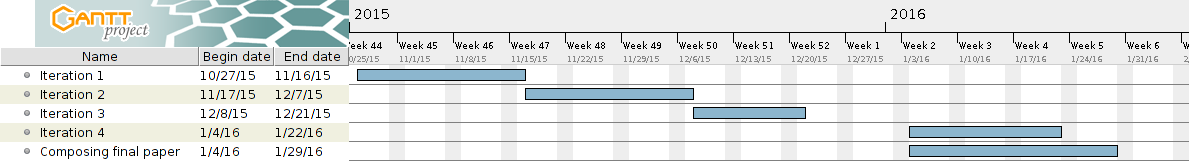
\includegraphics[width=1.0\linewidth]{gfx/chapter_4/hotpot_gantchart}
\caption[HotPot Gant chart]{BLP: HotPot Gant Chart}
\label{fig:hotpot_gantchart}
\end{figure}

The project has four iterations, each of which is three weeks long.

\begin{description}
\item[First iteration]
From 27/10/2015 to 16/11/2015
\begin{itemize}
\item Setup environment. 
\item Create initial DB schema. 
\item Create \emph{account} model with associated details. 
\item Create \emph{project} model. 
\item Add/remove accounts into/from projects. 
\item Create roles, security level. 
\item Assign account to many roles, and one security level.
\end{itemize}

\item[Second iteration]
From 17/11/2015 to 7/12/2015
\begin{itemize}
\item Create \emph{article} model.
\item Assigning security level and role to articles. 
\item Handling user login.
\item List projects related to current logged in account.
\item List articles related to current logged in account.
\end{itemize}

\item[Third iteration]
From 8/12/2015 to 29/12/2015
\begin{itemize}
\item Setup security logic on article actions (\eg create, view, list, edit, delete\dots). 
\item Create \emph{ticket} model. 
\item Apply security logic to ticket actions.
\end{itemize}

\item[Fourth iteration]
From 4/1/2016 to 31/1/2016
\begin{itemize}
\item Fix and update new security logics on \emph{objects' actions}.
\item Implement \emph{directory} structure for managing articles.
\item Apply graphical design.
\item Writing thesis documents and reports.
\end{itemize}
\end{description}
 
Every iterations has one or two days different from the planed schedule, however, in general, the programming part was completed as scheduled.

%----------------------------------------------------------------------------------------

\section{Technical information}
\label{ch:implementation:technical_information} 

In this section, I am going to introduce about the technologies used in this project, as well as the reason why I chose them at the first place.
The list below are technologies used in the project's developing environment:

\begin{description}
\item[OS] \emph{Ubuntu 14.04}.
It is a free, open source and widely used Linux distro developed by \emph{Canonical Ltd}.
It is easy to use, convenient, and strongly supported by a huge community.
I also used {Vagrant} (\emph{HashiCorp}) and \emph{VirtualBox} (\emph{Oracle}) for virtual environment.
\item[Programming language] \emph{Javascript - Nodejs}.
It is a very dynamic programming language which has an increasing number of developers.
This was my second project using Javascript on back-end, and it was the first project I work with back-end Javascript - Nodejs on my own. It was only for learning purpose, and indeed, I learned many things from this project.
\item[Framework and libraries] \emph{Expressjs, Sequelizejs}.
Expressjs may be the most popular web framework for Nodejs.
It has apparent documentation and a strong community.
Sequelizejs, on the other hand, is a famous and stable DAO library for Nodejs.
\item[Database] \emph{PostgreSQL} is my best choice of SQL Database.
It supports various data types and useful features.
Moreover, it has many libraries to be used in numerous programming language.
\item[Subversion control] \emph{Git} as the tool and \emph{GitHub} as the repository.
\item[Text Editors] \emph{Vim} for coding and \latex for composing thesis papers. And, as the \latex template, I use \emph{Classicthesis Typographic Thesis} of \emph{Andr\'{e} Miede}.

\end{description}

In fact, after finishing developing, a sample of the project has been deployed on a cloud machine at the address \href{http://178.62.253.47:3000/}{http://178.62.253.47:3000/}.
Most of the technical requirements are the same except that I used \emph{CentOS} (\emph{RedHat Inc} instead of Ubuntu for testing purpose and I can confirm that it works on \emph{CentOS} as well.
I can find every things needed on CentOS just like on Ubuntu.

%----------------------------------------------------------------------------------------

\section{Models}
\label{ch:implementation:models}

This section is a summary of my project's design.
I utilized MVC design model in this project.
All the logical controls will go to \emph{controllers}, which handle all the security policies as previously described in \autoref{ch:background:bell}.
So that, in this thesis document, I only focus explaining about the project's models and their relationship so that we can understand about the system's architecture.

In this section, I am going to list all the data models of the system.
We will learn about their properties, relations which will be illustrated as database diagrams.
\autoref{fig:er_diagram} is an \emph{ER diagram} including all data tables and their mutual relations in the system.

\begin{figure}[bth]                                                                                                                                                  
\myfloatalign
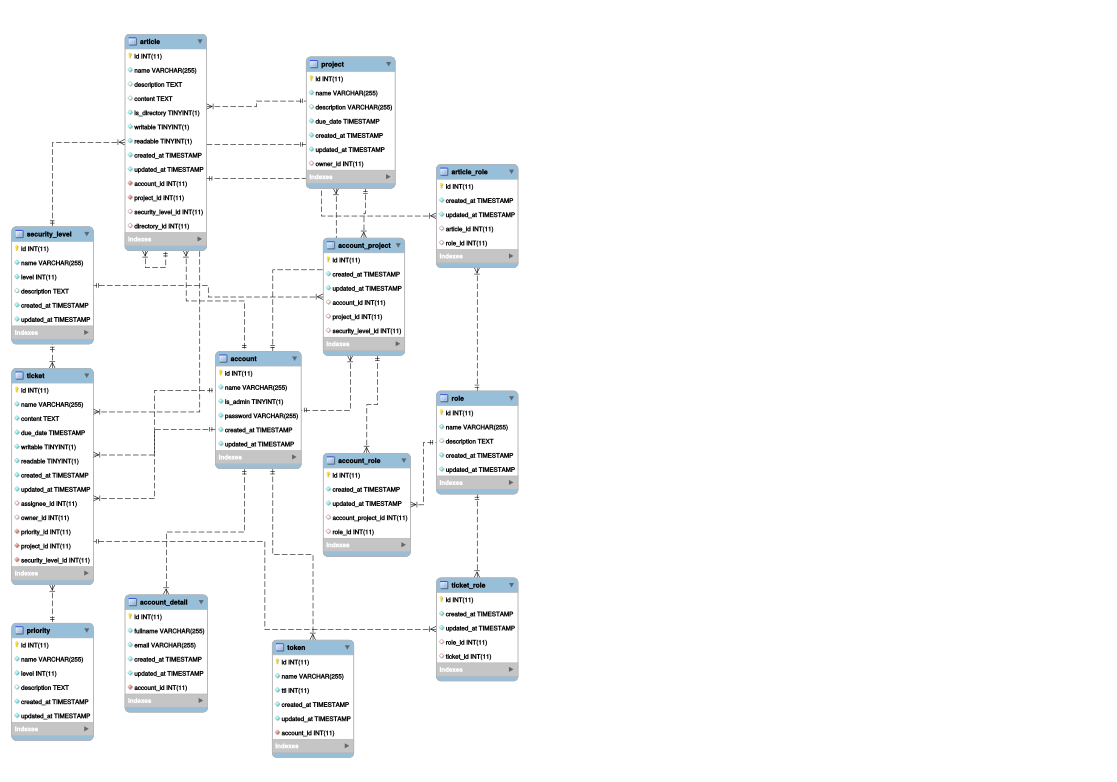
\includegraphics[width=1.0\linewidth]{gfx/chapter_4/er_diagram}
\caption[Entity Relation Diagram]{Entity Relation Diagram}
\label{fig:er_diagram}
\end{figure}
\clearpage

%------------------------------------------------

\subsection{Account}

\emph{Account} model corresponds to \emph{account subject} in the system.
It only consists of authentication and identity information of an account.
\autoref{tab:account_model_properties} explains all the properties of \emph{account} model, while \autoref{tab:account_model_relations} shows the relations between \emph{account} and the others in the system.

\begin{table}[!htbp]
\myfloatalign
\begin{tabularx}{\textwidth}{lXX} 
\toprule
\tableheadline{Property} & \tableheadline{Type} & \tableheadline{Description}\\ 
\midrule
\emph{name} &
string, not null, unique & 
The account's user name for logging in.\\
\midrule
\emph{password} & 
string, not null &
The account's password.\\
\midrule
\emph{password\_confirm} & 
string, not null &
This is a virtual field, which means it does not exist in the database table, and used for confirming password on account creation. \\
\midrule
\emph{is\_admin} & 
boolean, not null, default value: false &
Indicate whether an account is an administrator or not.\\
\bottomrule
\end{tabularx}
\caption[Account model properties.]{\emph{account} model properties.}  
\label{tab:account_model_properties}
\end{table}

\begin{table}[!htbp]
\myfloatalign
\begin{tabularx}{\textwidth}{llX} 
\toprule
\tableheadline{Model} & \tableheadline{Relation} & \tableheadline{Description}\\ 
\midrule
\emph{token} &
1:1 & 
Every account will have one new token for every logging in.\\
\midrule
\emph{account\_detail} & 
1:1 &
The account's detail information \eg full name, email, phone \dots \\
\midrule
\emph{project} & 
many:many &
An account may join many projects. 
This m:m relationship is defined through \emph{account\_project} model \ie relation table.\\
\midrule
\emph{account\_project} & 
1:many &
This is the relation model between \emph{account} and \emph{project} models to define the m:m relation.
In another word, it defines an account's \emph{project profiles}.
More about \emph{project profile} is explained in \autoref{ch:implementation:models:account_project} \\
\midrule
\emph{project} & 
1:many &
This relation is used for defining the account's \emph{owned projects}.
So once an account create a project, he will become that project's owner.\\
\midrule
\emph{article} & 
1:many &
This relation is used for defining the account's \emph{owned articles}.\\
\midrule
\emph{ticket} & 
1:many &
This relation is used for defining the account's \emph{owned tickets}.\\
\midrule
\emph{ticket} & 
1:many &
This relation is used for defining the account's \emph{assigned articles}.\\
\bottomrule
\end{tabularx}
\caption[Account model relations.]{Relations between \emph{account} and other models}  
\label{tab:account_model_relations}
\end{table}
\clearpage %to fix the float table problem.

%------------------------------------------------

\subsection{Account Detail}

This data model represents an account's detailed information. Its properties is listed in \autoref{tab:account_detail_model_properties}, and its relations to other models are explained in \autoref{tab:account_detail_model_relations}.

\begin{table}[!htbp]
\myfloatalign
\begin{tabularx}{\textwidth}{lXX} 
\toprule
\tableheadline{Property} & \tableheadline{Type} & \tableheadline{Description}\\ 
\midrule
\emph{fullname} &
string, not null, length between 8 and 128 & 
The account's fullname.\\
\midrule
\emph{email} & 
string, not null, unique &
The account's email address.\\
\bottomrule
\end{tabularx}
\caption[Account Detail model properties.]{\emph{account\_detail} model properties.}  
\label{tab:account_detail_model_properties}
\end{table}

\begin{table}[!htbp]
\myfloatalign
\begin{tabularx}{\textwidth}{llX} 
\toprule
\tableheadline{Model} & \tableheadline{Relation} & \tableheadline{Description}\\ 
\midrule
\emph{account} & 
1:1 &
One \emph{account\_detail} belongs to one \emph{account} and vice versa. \\
\bottomrule
\end{tabularx}
\caption[Account Detail model relations.]{Relations between \emph{account\_detail} and other models}  
\label{tab:account_detail_model_relations}
\end{table}
\clearpage %to fix the float table problem.

%------------------------------------------------

\subsection{Project}

This model contains all the information of a project. Its details are described in two table \autoref{tab:project_model_properties} and \autoref{tab:project_model_relations}

\begin{table}[!htbp]
\myfloatalign
\begin{tabularx}{\textwidth}{lXX} 
\toprule
\tableheadline{Property} & \tableheadline{Type} & \tableheadline{Description}\\ 
\midrule
\emph{name} &
string, not null, unique & 
The \emph{project}'s name.\\
\midrule
\emph{description} & 
string, allow null, length between 8 and 128  &
The \emph{project}'s description.\\
\midrule
\emph{due\_date} & 
date, allow null  &
The \emph{project}'s deadline.\\
\bottomrule
\end{tabularx}
\caption[Project model properties.]{\emph{project} model properties.}  
\label{tab:project_model_properties}
\end{table}

\begin{table}[!htbp]
\myfloatalign
\begin{tabularx}{\textwidth}{llX} 
\toprule
\tableheadline{Model} & \tableheadline{Relation} & \tableheadline{Description}\\ 
\midrule
\emph{account} & 
many:many &
A \emph{project} may have many \emph{members}. 
This m:m relationship is defined through \emph{account\_project} model. \\
\midrule
\emph{account} & 
many:1 &
This relation is used for defining the \emph{project}'s \emph{owner}.\\
\midrule
\emph{article} & 
1:many &
This relation is used for defining the \emph{project}'s \emph{articles}.\\
\midrule
\emph{ticket} & 
1:many &
This relation is used for defining the \emph{project}'s \emph{tickets}.\\
\bottomrule
\end{tabularx}
\caption[Project model relations.]{Relations between \emph{project} and other models}  
\label{tab:project_model_relations}
\end{table}
\clearpage %to fix the float table problem.

%------------------------------------------------

\subsection{Account Project (Project Profile)}
\label{ch:implementation:models:account_project}

\emph{account\_project} is a special model.
It is the relation table used to define the \emph{m:m} relation between \emph{account} and \emph{project} model.
Rather than that, it also contains all the information relating to a project of an account \eg his \emph{security level}, \emph{roles}.
In another word, this model contains all the security information of an account in a project, that we can use to authorize the account's access requests to the project's objects later.
In that manner, we also call this model a \emph{project\_profile} model.
Because this is only a relation model, there is no properties in it.
Its relations to other models are defined in \autoref{tab:account_project_model_relations}

\begin{table}[!htbp]
\myfloatalign
\begin{tabularx}{\textwidth}{llX} 
\toprule
\tableheadline{Model} & \tableheadline{Relation} & \tableheadline{Description}\\ 
\midrule
\emph{account} & 
many:many &
A project may have many \emph{members}. 
This m:m relationship is defined through \emph{account\_project} model. \\
\midrule
\emph{account} & 
1:1 &
This relation is used for defining the \emph{profile}'s \emph{account} (aka owner).\\
\midrule
\emph{project} & 
1:1 &
This relation is used for defining the \emph{profile}'s \emph{project}.\\
\midrule
\emph{security\_level} & 
1:1 &
This relation is used for defining the \emph{profile}'s \emph{security\_level}.\\
\midrule
\emph{role} & 
many:many &
This relation is used for defining the \emph{profile}'s \emph{roles}.
One profile may have many roles.\\
\bottomrule
\end{tabularx}
\caption[Account Project model relations.]{Relations between \emph{account\_project} and other models}  
\label{tab:account_project_model_relations}
\end{table}
\clearpage %to fix the float table problem.

%------------------------------------------------
\subsection{Security Level}

\emph{security\_level} model defines essential information of a security level label. Its details are described in two table \autoref{tab:security_model_properties} and \autoref{tab:security_model_relations}

\begin{table}[!htbp]
\myfloatalign
\begin{tabularx}{\textwidth}{lXX} 
\toprule
\tableheadline{Property} & \tableheadline{Type} & \tableheadline{Description}\\ 
\midrule
\emph{name} &
string, not null, unique & 
The \emph{security level}'s name.\\
\midrule
\emph{description} & 
string, allow null &
The \emph{security level}'s description.\\
\midrule
\emph{level} & 
integer, not null, unique &
The \emph{security level}'s level.
The higher value, the more important it is.\\
\bottomrule
\end{tabularx}
\caption[Security Level model properties.]{\emph{security\_level} model properties.}  
\label{tab:security_model_properties}
\end{table}

\begin{table}[!htbp]
\myfloatalign
\begin{tabularx}{\textwidth}{llX} 
\toprule
\tableheadline{Model} & \tableheadline{Relation} & \tableheadline{Description}\\ 
\midrule
\emph{account\_project} & 
1:many &
A \emph{security level} label may be used to tag on many \emph{accounts}.\\
\midrule
\emph{article} & 
1:many &
A \emph{security level} label may be used to tag on many \emph{articles}.\\
\midrule
\emph{ticket} & 
1:many &
A \emph{security level} label may be used to tag on many \emph{articles}.\\
\bottomrule
\end{tabularx}
\caption[Security Level model relations.]{Relations between \emph{security\_level} and other models}  
\label{tab:security_model_relations}
\end{table}
\clearpage %to fix the float table problem.

%------------------------------------------------

\subsection{Role}

\emph{role} model defines essential information of a role label.
Its details are described in two table \autoref{tab:role_model_properties} and \autoref{tab:role_model_relations}

\begin{table}[!htbp]
\myfloatalign
\begin{tabularx}{\textwidth}{lXX} 
\toprule
\tableheadline{Property} & \tableheadline{Type} & \tableheadline{Description}\\ 
\midrule
\emph{name} &
string, not null, unique & 
The \emph{role}'s name.\\
\midrule
\emph{description} & 
string, allow null &
The \emph{role}'s description.\\
\bottomrule
\end{tabularx}
\caption[Role model properties.]{\emph{role} model properties.}  
\label{tab:role_model_properties}
\end{table}

\begin{table}[!htbp]
\myfloatalign
\begin{tabularx}{\textwidth}{llX} 
\toprule
\tableheadline{Model} & \tableheadline{Relation} & \tableheadline{Description}\\ 
\midrule
\emph{account\_project} & 
many:many &
One or many \emph{role} labels may be used to tag on many \emph{profiles}.
This relation is defined through \emph{account\_role} model.\\
\midrule
\emph{article} & 
many:many &
One or many \emph{role} labels may be used to tag on many \emph{articles}.
This relation is defined through \emph{article\_role} model.\\
\midrule
\emph{ticket} & 
many:many &
One or many \emph{role} labels may be used to tag on many \emph{articles}.
This relation is defined through \emph{ticket\_role} model.\\
\bottomrule
\end{tabularx}
\caption[Role model relations.]{Relations between \emph{role} and other models}  
\label{tab:role_model_relations}
\end{table}
\clearpage %to fix the float table problem.

%------------------------------------------------

\subsection{Article}

\emph{article} model defines essential information of an article.
Its details are described in two table \autoref{tab:article_model_properties} and \autoref{tab:article_model_relations}

\begin{table}[!htbp]
\myfloatalign
\begin{tabularx}{\textwidth}{lXX} 
\toprule
\tableheadline{Property} & \tableheadline{Type} & \tableheadline{Description}\\ 
\midrule
\emph{name} &
string, not null & 
The \emph{article}'s name.\\
\midrule
\emph{description} & 
string, allow null &
The \emph{article}'s description.\\
\midrule
\emph{content} & 
string, allow null &
The \emph{article}'s content.\\
\midrule
\emph{is\_directory} & 
boolean, not null, default false &
Indicate whether this article is a directory or not.\\
\midrule
\emph{writable} & 
boolean, not null, default false &
Indicate whether this article is writable or not.\\
\midrule
\emph{readable} & 
boolean, not null, default false &
Indicate whether this article is readable or not.\\
\bottomrule
\end{tabularx}
\caption[Article model properties.]{\emph{article} model properties.}  
\label{tab:article_model_properties}
\end{table}

\begin{table}[!htbp]
\myfloatalign
\begin{tabularx}{\textwidth}{llX} 
\toprule
\tableheadline{Model} & \tableheadline{Relation} & \tableheadline{Description}\\ 
\midrule
\emph{account} & 
many:1 &
This relation is used for defining the \emph{article}'s \emph{owner}.\\
\midrule
\emph{project} & 
many:1 &
This relation is used for defining in which \emph{project} the \emph{article} belongs to.\\
\midrule
\emph{roles} & 
many:many &
An \emph{article} may have one or many \emph{role} labels.
This relation is defined through \emph{article\_role} model.\\
\midrule
\emph{security\_level} & 
many:1 &
This relation is used for defining the \emph{article}'s \emph{security level} label.\\
\midrule
\emph{article} & 
1:many &
If this \emph{article} is a directory, this relation defines \emph{articles} belong to it.\\
\midrule
\emph{article} & 
many:1 &
This relation is used for defining the \emph{article}'s \emph{directory} if available.\\
\bottomrule
\end{tabularx}
\caption[Article model relations.]{Relations between \emph{article} and other models}  
\label{tab:article_model_relations}
\end{table}
\clearpage %to fix the float table problem.

%------------------------------------------------

\subsection{Priority}

\emph{priority} is a property of \emph{ticket} model.
So, in order to provide a scalable system, I added this table for users to insert the suitable priorities for their system.
This model defines essential information of a priority.
Its details are described in two table \autoref{tab:priority_model_properties} and \autoref{tab:priority_model_relations}

\begin{table}[!htbp]
\myfloatalign
\begin{tabularx}{\textwidth}{lXX} 
\toprule
\tableheadline{Property} & \tableheadline{Type} & \tableheadline{Description}\\ 
\midrule
\emph{name} &
string, not null, unique & 
The \emph{priority}'s name.\\
\midrule
\emph{description} & 
string, allow null &
The \emph{priority}'s description.\\
\midrule
\emph{level} & 
integer, not null, unique &
The \emph{priority}'s level.
The higher level, the higher priority.\\
\bottomrule
\end{tabularx}
\caption[Priority model properties.]{\emph{priority} model properties.}  
\label{tab:priority_model_properties}
\end{table}

\begin{table}[!htbp]
\myfloatalign
\begin{tabularx}{\textwidth}{llX} 
\toprule
\tableheadline{Model} & \tableheadline{Relation} & \tableheadline{Description}\\ 
\midrule
\emph{ticket} & 
1:many &
This relation is used for defining \emph{tickets} with the \emph{priority}.\\
\bottomrule
\end{tabularx}
\caption[Priority model relations.]{Relations between \emph{priority} and other models}  
\label{tab:priority_model_relations}
\end{table}
\clearpage %to fix the float table problem.

%------------------------------------------------

\subsection{Ticket}

\emph{ticket} model defines essential information of an ticket.
Its details are described in two table \autoref{tab:ticket_model_properties} and \autoref{tab:ticket_model_relations}

\begin{table}[!htbp]
\myfloatalign
\begin{tabularx}{\textwidth}{lXX} 
\toprule
\tableheadline{Property} & \tableheadline{Type} & \tableheadline{Description}\\ 
\midrule
\emph{name} &
string, not null & 
The \emph{ticket}'s name.\\
\midrule
\emph{content} & 
string, not null &
The \emph{ticket}'s content.\\
\midrule
\emph{due\_date} & 
date, allow null &
The \emph{ticket}'s deadline.\\
\midrule
\emph{writable} & 
boolean, not null, default false &
Indicate whether this ticket is writable or not.\\
\midrule
\emph{readable} & 
boolean, not null, default false &
Indicate whether this ticket is readable or not.\\
\bottomrule
\end{tabularx}
\caption[Ticket model properties.]{\emph{ticket} model properties.}  
\label{tab:ticket_model_properties}
\end{table}

\begin{table}[!htbp]
\myfloatalign
\begin{tabularx}{\textwidth}{llX} 
\toprule
\tableheadline{Model} & \tableheadline{Relation} & \tableheadline{Description}\\ 
\midrule
\emph{account} & 
many:1 &
This relation is used for defining the \emph{ticket}'s \emph{owner}.\\
\midrule
\emph{account} & 
many:1 &
This relation is used for defining the \emph{ticket}'s \emph{assignee}.\\
\midrule
\emph{project} & 
many:1 &
This relation is used for defining in which \emph{project} the \emph{ticket} belongs to.\\
\midrule
\emph{roles} & 
many:many &
An \emph{ticket} may have one or many \emph{role} labels.
This relation is defined through \emph{ticket\_role} model.\\
\midrule
\emph{security\_level} & 
many:1 &
This relation is used for defining the \emph{ticket}'s \emph{security level} label.\\
\midrule
\emph{priority} & 
1:many &
This relation is used for defining the \emph{ticket}'s \emph{priority} label.\\
\bottomrule
\end{tabularx}
\caption[Ticket model relations.]{Relations between \emph{ticket} and other models}  
\label{tab:ticket_model_relations}
\end{table}
\clearpage %to fix the float table problem.

%----------------------------------------------------------------------------------------
